%%%%%%%%%%%%%%%%%%%%%%%%%%%%%%%%%%%%%%%%%%%%%%%%%%%%%%%%%%%%%%%%%%%%%%%%%%
%%%%%%%%%%%%   CAPTER 2   %%%%%%%%%%%%%%%%%%%%%%%%%%%%%%%%%%%%%%%%%%%%%%%%
%%%%%%%%%%%%%%%%%%%%%%%%%%%%%%%%%%%%%%%%%%%%%%%%%%%%%%%%%%%%%%%%%%%%%%%%%%
\chapter{Background and Related Work}
\label{chap:bg_related_work}
Minimizing size, weight and power consumption of the Radar processor without compromising performance is the topic under research. Low cost and portable Radar processor is intended for weight and power limited airborne platform such as Unmanned Airborne Vehicles \cite{uav}. On satisfactory performance, this may open doors for new business opportunities in Radar processing and safety critical applications. ARM is the favourable architecture in this regard, and has been running in millions of smart phones, tablets and portable gadgets. Instead of one high capacity, power hungry, bulk processor, several small, energy efficient, compact processors of ARM type can be deployed. The way of grouping the processors, experiment setup \footnote{These information are based on the technical documentation provided by Airbus Defence and Space GmbH, titled \textsl{Future Combat Air System - Analysis of IMA Modules,} version B.} and state of the art related work are elaborated in this chapter.

%%%%%%%%%%%%%%%%%%%%%%%%%%%%%%%%%%%%%
%%%%%%%%%%%%%%%%%%%%%%%%%%%%%%%%%%%%%
%%%%%%%%%%%%   SECTION   %%%%%%%%%%%%
%%%%%%%%%%%%%%%%%%%%%%%%%%%%%%%%%%%%%
%%%%%%%%%%%%%%%%%%%%%%%%%%%%%%%%%%%%%
\section{IMA Processor Architecture} 
\label{sec:bg_related_work:ima}
Integrated Modular Avionics is the cluster of real-time computing elements capable of executing multiple tasks having different safety critical levels. Instead of several dedicated computers for different purposes, a common hardware platform for many systems is used. This improves fault isolation, increased airborne functionality and ability to move applications between standardized computers \cite{theAvionics}. To comply with the environmental requirements, industrial temperature standard, MCIMX6Q7CVT08AC processor type with 800MHz clock speed is used. \\

IMA architecture comprises of the following modules \footnote{SPM Module and iCON Module are out of this thesis scope.}
\begin{compactitem} 
	\item up to 2 Platform Support Modules (PSM) 
	\item up to 6 Data Graphics Processing Module (DGPM) or Signal Processing Module (SPM) or any combination of these two.
	\item up to 3 Interface Concentrator Module (iCON).
	\item a rack backplane.
\end{compactitem}

%%%%%%%%%%%%%%%%%%%%%%%%%
%%%%%   SUB-SECTION   %%%
%%%%%%%%%%%%%%%%%%%%%%%%%
%%%%%%%%%%%%%%%%%%%%%%%%%
\subsection{Platform Support Modules (PSM)}
\label{ss:bg_related_work:psm}
The PSM has the following components:
\begin{compactitem} 
	\item one iMX6Q CPU, clocked 800MHz.
	\item one 1GBit/s-Ethernet switch with 10 bi-directional communication ports.
	\item CPU has it's own private 4GiB SDRAM and non-volatile NOR/NAND Flash memory.
	\item 16GiB Solid State Disk, connected to the CPU via SATA interface.
\end{compactitem}

\begin{figure}[h!]
	\centering
	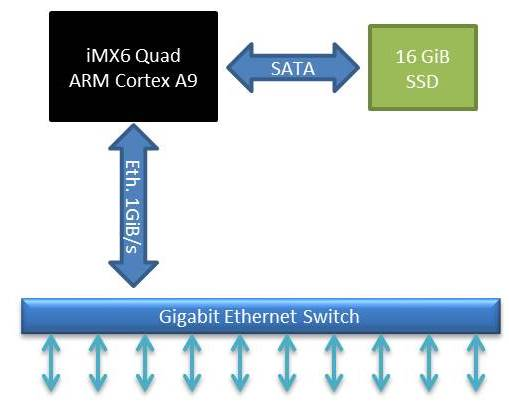
\includegraphics[width=90mm]{figures/psm}
	\caption{Platform Support Module \cite{fcas}}
	\label{fig:bg_related_work:ima:psm}
\end{figure}

The PSM Module acts as a router between different modules of the Radar processor. It directs the Radar raw data to an apt processing module (DGPM or SPM) and send the processing result to a target display module.

%%%%%%%%%%%%%%%%%%%%%%%%%
%%%%%   SUB-SECTION   %%%
%%%%%%%%%%%%%%%%%%%%%%%%%
\subsection{Data Graphics Processing Module (DGPM)}
\label{ss:bg_related_work:dgpm}
The DGPM has the following characteristics:
\begin{compactitem} 
	\item 4 iMX6Q CPUs, clocked 800MHz.
	\item one 1GBit/s-Ethernet switch with 6 bi-directional communication ports.
	\item each of the 4 CPUs has it's own private 4GiB SDRAM and non-volatile NOR/NAND Flash.
memory \\
\end{compactitem}

\begin{figure}[h!]
	\centering
	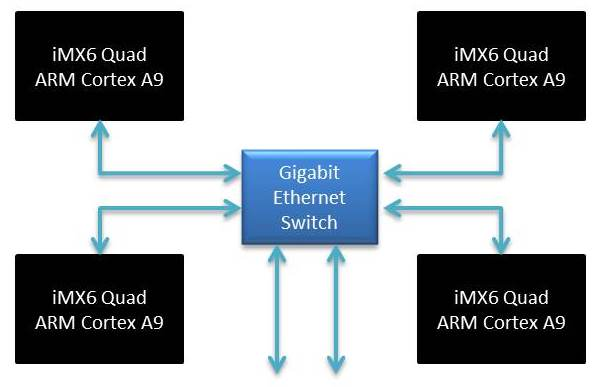
\includegraphics[width=100mm]{figures/dgpm}
	\caption{Data Graphics Processing Module \cite{fcas}}
	\label{fig:bg_related_work:ima:dgpm}
\end{figure}

The iMX6Q6 CPU has four identical ARM Cortex A9 cores with Advanced SIMD unit (NEON), 32KiB I and D-cache, one unified 1MiB L2-cache shared by 4 cores, smart DMA, 3D and 2D Graphics Processing Unit, one common 533MHz 64-bit DDR3 memory interface, one common 1GBit/s Ethernet interface and several other standard interfaces \cite{imx_spec}, (Appendix \ref{app:imx6q}). The SPM Module has not been considered due to the decision of Airbus DS.

%%%%%%%%%%%%%%%%%%%%%%%%%
%%%%%   SUB-SECTION   %%%
%%%%%%%%%%%%%%%%%%%%%%%%%
\subsection{Radar Processor Design}
\label{ss:bg_related_work:togther}
As shown in Figure \ref{fig:bg_related_work:ima:radar_processor}, the received raw data will undergo the following stages to be transformed as desired information.
\begin{enumerate}
	\item Radar receiver front-end sends the received data to the iCON1 Module along with supplementary information like antenna azimuth, antenna elevation, etc. Data distribution to the PSM modules is controlled by the iCON1. 

	\item PSM1 and PSM2 routes the received data to the pre-defined DGPM modules. Routing mechanism can be reconfigured.

	\item As soon as the DGPM has completed processing, data will be sent back to the respective PSM module.

	\item PSM routes the processed data to iCON2. 

	\item iCON2 routes the processed A/A Mode data, SAR Mode data to the tracking processor, display processor respectively. 
\end{enumerate}
Nominal data transfer rate of the communication links are 1GBit/s. Booting the software can be done from SSD or remotely via an appropriate system interface.

\begin{figure}[h!]
	\centering
	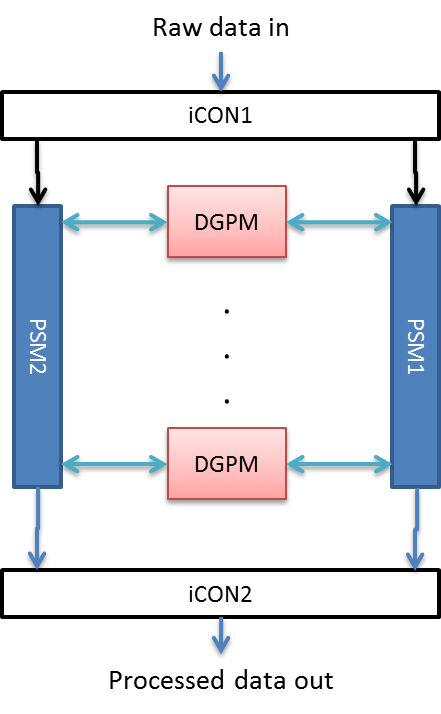
\includegraphics[]{figures/radar_processor}
	\caption{Block Diagram of Radar Processor \cite{fcas}}
	\label{fig:bg_related_work:ima:radar_processor}
\end{figure}

\lstset{ %
  backgroundcolor=\color{mildyellow},   % choose the background color; you must add \usepackage{color} or \usepackage{xcolor}
  breakatwhitespace=false,         % sets if automatic breaks should only happen at whitespace
  breaklines=true,                 % sets automatic line breaking
  keepspaces=true,                 % keeps spaces in text, useful for keeping indentation of code (possibly needs columns=flexible)
  numbers=none,                    % where to put the line-numbers; possible values are (none, left, right)
  showspaces=false,                % show spaces everywhere adding particular underscores; it overrides 'showstringspaces'
  showstringspaces=false,          % underline spaces within strings only
  basicstyle=\ttfamily\small,
  frame=single,
}

%%%%%%%%%%%%%%%%%%%%%%%%%%%%%%%%%%%%%
%%%%%%%%%%%%%%%%%%%%%%%%%%%%%%%%%%%%%
%%%%%%%%%%%%   SECTION   %%%%%%%%%%%%
%%%%%%%%%%%%%%%%%%%%%%%%%%%%%%%%%%%%%
%%%%%%%%%%%%%%%%%%%%%%%%%%%%%%%%%%%%%
\section{Air to Air Mode Processing Chain}
\label{sec:bg_related_work:proc_chain}
Previous work has been carried out by Airbus DS in Future Combat Air System (FCAS) project, see \cite{fcas}. This section is an excerpt of the FCAS project, describes the Radar processing chain to understand the rest of the thesis.

At first, the Radar system in the flight scans the sky $\pm$60$^{\circ}$ from bore-sight. The azimuth scan of the antenna is sub-divided into 2 x 5 angular segments, called look directions (5 segments in the positive half and 5 segments in the negative half of the scan width). Given the beam width of 2.5$^{\circ}$, 48 beams are required to cover the 120$^{\circ}$ space. Antenna's gain is high along the bore-sight direction \cite{boreSight}\cite{bsTR}. So, the look directions adjacent to the bore-sights have 4 beams each and the remaining 8 look directions have 5 beams each, counting 48 beams totally. Figure \ref{fig:bg_related_work:aa_look_dir} explains the 5 look direction segments in positive half of the azimuth scan. The Air to Air Mode has different PRF set for different look directions. The PRF and range gate configuration determines the amount of input data to the Radar processor. Table \ref{tbl:aa_exe} shows the maximum execution time of the Radar functions running on a single core, 1GHz iMX6Quad processor. The baseline analysis scales down the results to 800MHz to match the IMA processor architecture.

\begin{figure}[h!]
	\centering
	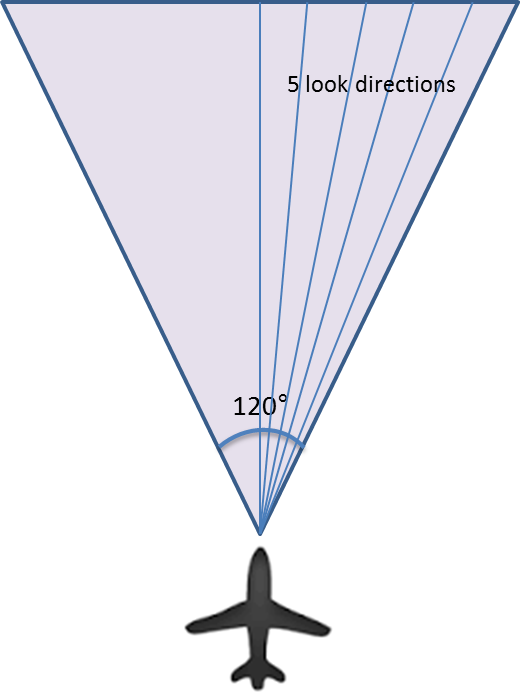
\includegraphics[width=55mm]{figures/look_dir}
	\caption{Details of the A/A Mode Scan}
	\label{fig:bg_related_work:aa_look_dir}
\end{figure}

The Radar antenna has 8 transmit and receive channels and 1 guard channel. The guard channel works as a detector to distinguish main-lobe echoes and side-lobe echoes. Every scan consists several Dwells. All the Dwells are independent. The A/A Mode processing is done independently for each Dwell. It comprises of the following stages.\footnote{This section only describes an overview of the algorithm, since the algorithm is classified as Airbus DS Confidential.}

\begin{figure}[h!]
	\centering
	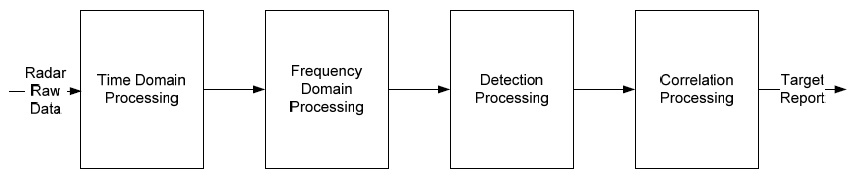
\includegraphics[width=160mm]{figures/aa_block_dia}
	\caption{Block Diagram of Air to Air Mode Processing}
	\label{fig:bg_related_work:aa_block_dia}
\end{figure}

\subsection{Time Domain Processing}
Beam-forming is a Digital Signal Processing technique that allows the Radar antenna to focus on a particular direction \cite{beamforming}. Beam-forming has to be performed for Sum channel($S_{S}$), Azimuth channel($S_{AZ}$) and Elevation channel($S_{EL}$). During Sum channel beam-forming, the input vectors of 8 antenna receive channels are multiplied with pre-calculated Sum channel beam-forming vectors. The resulting vectors are added to produce a Sum channel beam. This step is repeated for Azimuth channel and Elevation channel. Guard (9$^{th}$) channel doesn't require beam-forming, only requires float conversion. Each of the processed four channel data are multiplied by pre-calculated weighting vector. 

Digital Pulse Compression, also called Convolution, is computation expensive in time domain, so it is performed in frequency domain. Convolution in time domain is multiplication in frequency domain, it is performed channel by channel by computing FFT, Multiplication followed by IFFT.

\begin{figure}[h!]
	\centering
	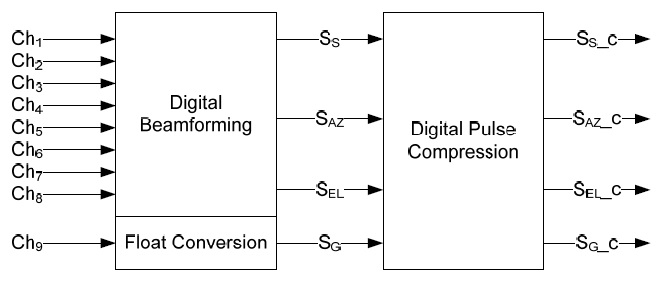
\includegraphics[width=120mm]{figures/aa_tdp}
	\caption{A/A Mode Time Domain Processing}
	\label{fig:bg_related_work:aa_tdp}
\end{figure}

\subsection{Frequency Domain Processing (FDP)}
Each channel pulse compressed data is in the form of [pulse x range] matrix. Frequency domain transformation has to be applied on the data corresponding to the same range gates of different pulse. So the pulse compressed data shall be corner turned to [range x pulse] matrix as shown in Figure \ref{fig:bg_related_work:cot}.

\begin{figure}[h!]
	\centering
	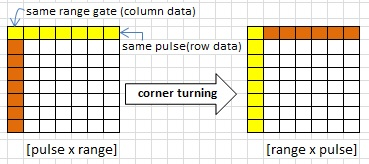
\includegraphics[width=90mm]{figures/cot}
	\caption{Corner Turning}
	\label{fig:bg_related_work:cot}
\end{figure}
\FloatBarrier
\begin{figure}[h!]
	\centering
	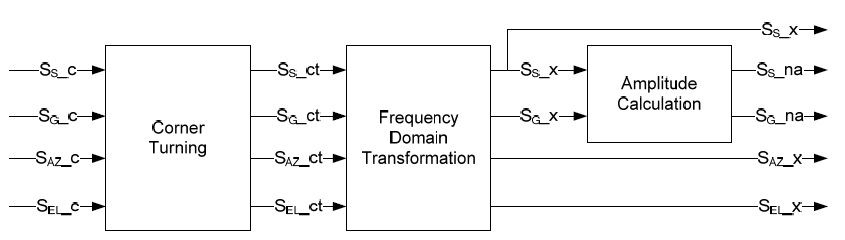
\includegraphics[width=140mm]{figures/aa_fdp}
	\caption{A/A Mode Frequency Domain Processing}
	\label{fig:bg_related_work:aa_fdp}
\end{figure}
FFT is computed for the Sum, Guard, Azimuth and Elevation channel followed by magnitude of the Sum channel and Guard channel are computed on the corner turned data..

\subsection{Detection Processing (DET)}
Area threshold of the individual elements in the Sum channel and the Guard channel are determined by computing average of the surrounding elements values. An additional pre-alarm matrix is computed by comparing the amplitude matrix and the area threshold matrix. The pre-alarm says the detection may be a potential target. If the element in the amplitude matrix is greater than the corresponding element in the threshold matrix, pre-alarm is set TRUE in the corresponding pre-alarm matrix, otherwise pre-alarm element is set to FALSE. To prevent the Sum channel alarms caused by side-lobe entries, it is compared with the Guard channel alarms. \\The number of alarms are limited by the N$_{max\_alarms}$ with the shortest range from the list called Constant False Alarm Rate(CFAR). Alarm list is generated by referring the pre-alarm matrix and corresponding Sum, Azimuth, Elevation channel values.

\begin{figure}[h!]
	\centering
	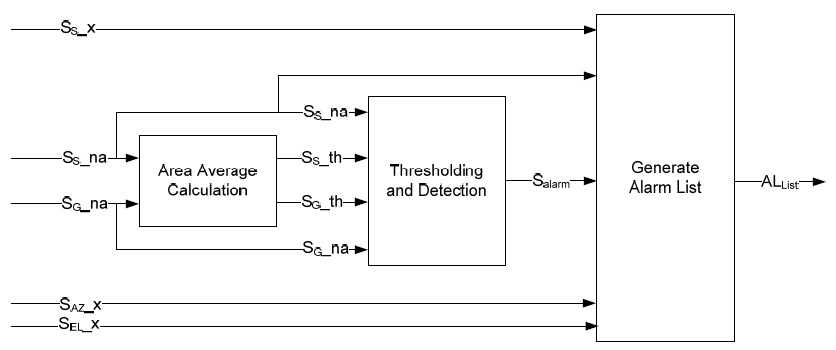
\includegraphics[width=140mm]{figures/aa_det}
	\caption{A/A Mode Detection Processing}
	\label{fig:bg_related_work:aa_det}
\end{figure}


\subsection{Correlation Processing}
This stage resolves the ambiguity in distance and velocity by comparing the current burst data with 7 previous bursts. Correlation processing is not considered as a performance critical module and hence this stage is not benchmarked. 

\begin{figure}[h!]
	\centering
	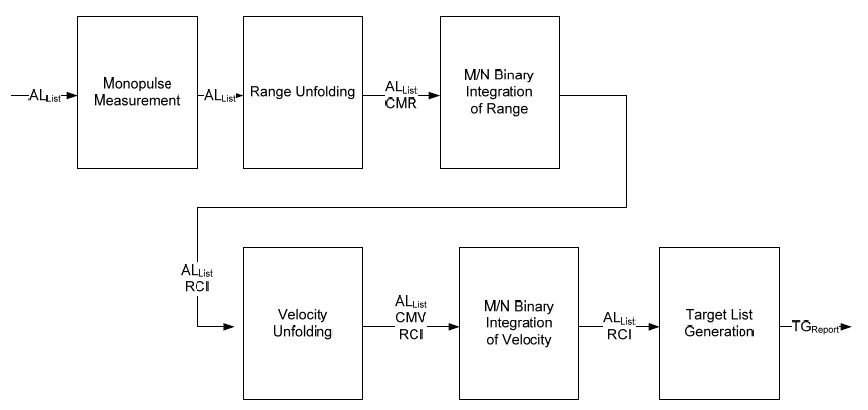
\includegraphics[width=140mm]{figures/aa_corr}
	\caption{A/A Mode Correlation Processing}
	\label{fig:bg_related_work:aa_corr}
\end{figure}
\FloatBarrier

\section{A/A Mode Sequence of Execution}
\label{sec:ch2:benchmark_results}
Performance critical functions related to the Radar processing algorithm are identified by Airbus DS. The functional blocks are executed in the iMX6Quad processor, clocked 1GHz and their execution times are listed in Table \ref{tbl:aa_exe}. The functional block 100CMYACC8, multiplies each element of a [100 x 8] element complex matrix with an 8-element complex vector and accumulate the 8 complex multiplication results to a single complex result, resulting in a [100 x 1] element complex matrix. Explanation about the other functional blocks can be found in Appendix \ref{description:benchmark}.

\begin{longtable}{|l|l|l|}
		\hline
		\textbf{Functional Block} & \textbf{\#cycles in iMX6Quad processor} & \textbf{Unit}  \TBstrut \\ \hline
		100CMYACC8 & 79 & per 8 element \TBstrut \\ \hline
		100RMY50 & 15 & per complex element \TBstrut \\ \hline
		100CONV128 & 24100 & per 128-pt vector \TBstrut \\ \hline
		150COT50 & 12 & per complex element \TBstrut \\ \hline
		100FFT64 & 2,550 & per 64-pt vector \TBstrut \\ \hline
		50MAG256 & 20 & per complex element \TBstrut \\ \hline
		64AVG100 & 20 & per element \TBstrut \\ \hline
		64CMPR100 & 7 & per element \TBstrut \\ \hline
		64DET100 & 10 & per element  \TBstrut \\ \hline
		\caption{Measured Execution Cycles of the Functional Blocks}
		\label{tbl:aa_exe}
\end{longtable}

The functional blocks shall be executed as shown in Figure \ref{fig:bg_related_work:aa_seq} to mimic the Radar processing chain. Functions of the Correlation processing are not included here. In the following figure, \textsl{3x CMYACC} means, computing \hyperlink{benchmarks}{CMYACC} for three channels ($S_{S},S_{AZ},S_{EL}$).

\begin{figure}[h!]
	\centering
	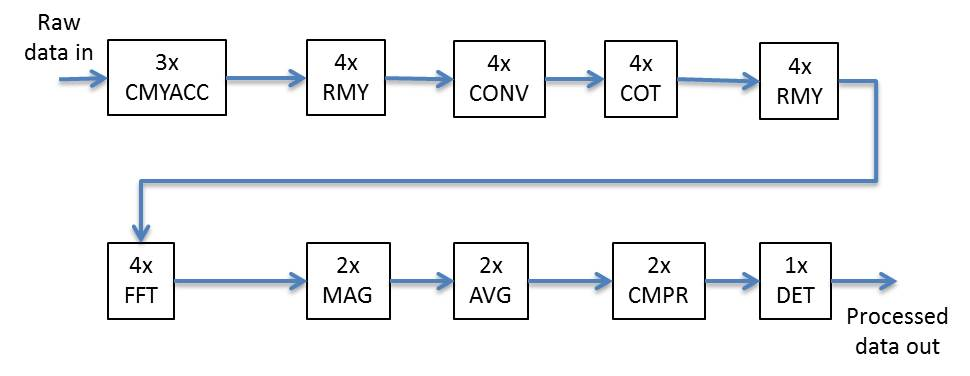
\includegraphics[width=160mm]{figures/aa_seq}
	\caption{A/A Mode, Sequence of Functional Blocks Execution}
	\label{fig:bg_related_work:aa_seq}
\end{figure}

STREAM benchmark\cite{McCalpin2007} is used to measure memory bandwidth of a machine. The STREAM benchmark is a simple, synthetic benchmark designed to measure sustainable memory bandwidth (in MiB/s) and a corresponding computation rate for four simple vector kernels namely Copy, Scale, Add and Triad \cite{streamDef}. According to the STREAM benchmark, 400 MiB/s data transfer rate is measured while copying data from one memory location of the SDRAM to another memory location, when a single core is active (2cycle/byte). L2 cache to SDRAM data transfer rate of 350MiB/s (2.29cycle/byte) is measured when all the four cores are active. Operating System overhead is assumed as the factor of 1.3 to carry out the execution. Cycle time of the core is 1.25ns, as it is running at 800MHz frequency. Execution cycle for the Correlation processing is heuristically assumed as follows.


\begin{table}[h!]
	\centering
	\begin{tabular}{|l|l|l||l|l|} 
	 	\hline
		\textbf{Process} & \textbf{\#cycles} & \textbf{Unit} & \textbf{\#cycles} & \textbf{Unit}  \\ \hline
		Monopulse Measurement & 500 & per alarm & - & - \\ \hline
		Range Unfolding & 30 & per range gate & 200 & per alarm \\ \hline
		M/N Binary Integration of Range & 40 & per range gate & 500 & per alarm \\ \hline
		Velocity Unfolding & 30 & per alarm & - & - \\ \hline
		M/N Binary Integration of Velocity & 80 & per alarm & - & - \\ \hline
		Target List Generation & 100 & per target & - & - \\ \hline
	\end{tabular}
	\caption{Execution Cycle of Correlation Processing \cite{fcas}}
	\label{tbl:rel_work:corr_proc_exe}
\end{table}

The execution cycle results listed in the Tables \ref{tbl:rel_work:corr_proc_exe} and \ref{tbl:aa_exe} are the fundamentals for the baseline analysis, explained in the next chapter.
 
%%%%%%%%%%%%%%%%%%%%%%%%%%%%%%%%%%%%%
%%%%%%%%%%%%%%%%%%%%%%%%%%%%%%%%%%%%%
%%%%%%%%%%%%   SECTION   %%%%%%%%%%%%
%%%%%%%%%%%%%%%%%%%%%%%%%%%%%%%%%%%%%
%%%%%%%%%%%%%%%%%%%%%%%%%%%%%%%%%%%%%
\section{Air to Air Mode Radar Characteristics}
\label{ss:aa_mode:radar_char}
Air to Air Mode Radar has the following characteristics. The transmitted carrier frequency is 9GHz and it can detect targets in 40nm range, moving at velocity $\pm$3Mach. A burst shall have a maximum of 32 alarms and a maximum of 16 targets, formed out of the 32 alarms. That is, a burst shall have maximum of 32 detections, of which 16 can be real targets.

\begin{table}
	\centering
	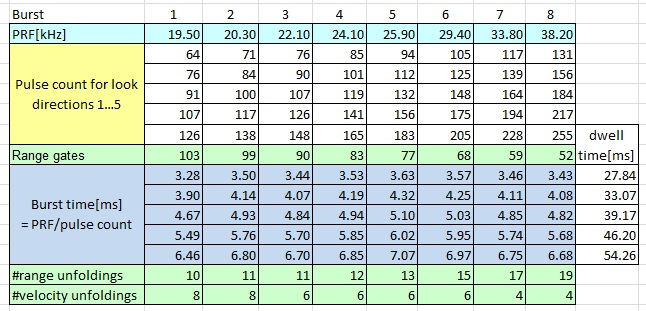
\includegraphics[width=140mm]{figures/aa_char}
	\caption{A/A Mode Radar Characteristics}
	\label{fig:bg_related_work:aa_char}
\end{table}

Table \ref{fig:bg_related_work:aa_char} shows the detailed information of the Radar system. The first burst of the Look direction-1 consists of 64 pulses transmitted at 19.5 KHz frequency and every pulse shall have 103 range gates. Range unfolding and Velocity unfolding are performed to compute the unambiguous range and unambiguous velocity of the target respectively. They can be mathematically calculated as follows \cite{unambiVelo}. 

\begin{align*}
	\label{equ:burst_time_calc}
	Dwell \enspace time &= \sum\limits_{n=1}^{8} Burst \enspace time_{n} \\[0.3cm]
	Unambiguous \: Range &= \frac{1}{2} \: \frac{velocity \: of \: the \: radar \: signal}{PRF \: frequency} \\[0.3cm]
	Range \: Unfoldings &= \frac{max.range}{unambiguous \: range} \\[0.3cm]
	Unambiguous \: Velocity &= \frac{1}{2} \frac{velocity \: of \: the \: radar \: signal}{carrier \: frequency} * PRF \: frequency \\[0.3cm]
	Velocity \: unfolding &= 2 * ROUNDUP \bigg( \frac{max.velocity}{unambiguous \: velocity} \bigg ) \\[0.3cm] \stepcounter{equation}\tag{\theequation} 
\end{align*}

Active Electronically Scanned Array (AESA) Radar is an airborne Radar, capable of steering beams rapidly \cite{aesaAbt}. In case of AESA Radar, processing latency influences agility of the system. Beam steering is performed electronically in AESA Radar compared to the mechanical steering in conventional Radars. Dynamic carrier frequency and PRF characteristics of the AESA Radar makes it hard to be intercepted by Radar Warning Receiver \cite{aesaIntercept}.

%%%%%%%%%%%%%%%%%%%%%%%%%%%%%%%%%%%%%
%%%%%%%%%%%%%%%%%%%%%%%%%%%%%%%%%%%%%
%%%%%%%%%%%%   SECTION   %%%%%%%%%%%%
%%%%%%%%%%%%%%%%%%%%%%%%%%%%%%%%%%%%%
%%%%%%%%%%%%%%%%%%%%%%%%%%%%%%%%%%%%%
\section{Related Work}
\label{sec:related_work}
Deploying ARM processors in fighter aircraft is in the research stage at the moment. Footprints of the low cost Radar processor and optimal scheduling algorithm have been considered as related work of this thesis. Many innovative architectures have been investigated in past to reduce the size, weight and power(SWaP) requirements of the Radar processor. Some of them are discussed below.

In continuation to the bird strike happened in Alaska, a low cost Radar system "eBirdRad" is developed by Tim J. Nohara, et al \cite{relWork1}, focused to detect birds activity in the sky. The Radar uses X-band frequency, 4$^{\circ}$ beam width, 10m resolution, covering 360$^{\circ}$  azimuth angle and 6nm distance. Proprietary Accipiter Radar processor is used for computations. eBirdRad could detect the birds in real time though there are rooms for improvement. It doesn't aim to reduce weight and power requirements, hence it is not a perfect rival for ARM based Radar processors. 

Salama Y, Fitzgerald D et al \cite{relWork3}, have used Wafer Scale Signal Processor(WSSP) for power efficient Radar signal processing. WSSP is a general purpose floating point processor with 4FLOPS/cycle peak performance, consuming 2 to 10 GFLOPS/watt roughly. Simulation results of FFT benchmark shows that up to 3.2FLOPS/cycle can be utilized for 100k FFT size. The WSSP processor has made efforts to reduce power requirements, disregarding size, weight and cost factors.

Research has hit the industry with \textsl{Programmable DSP Cores for Radar Processing}. APTCORE \cite{relWork4}, uses patented processor architecture to efficiently process the Radar benchmarks. It claims to have 3.3x energy efficiency in FFT processing compared to the standard DSPs. According to the documentation, it is compact, low cost, lowest power, scalable and highly configurable. In addition, range and direction processing of 10 sets of 512 values across 16 antennas take 2.3ms at a clock speed of 200MHz. Although the APTCORE has impressive performance in the product brief document, further investigation is required to compare it against ARM Cortex A9's performance.

ARM type processor has been used by Zeng Y, Xu J and Peng D in Velocity Measuring System \cite{relWork2}. Implementation is done in assembly language to take advantage of the pipeline. It uses 24GHz frequency waves and can track the vehicle velocities from 5km/h to 250km/h in 1.5km range. It is a low cost, low power, compact system meant for traffic management.

Cheng C, Chien-Chung C et al \cite{RTsched} proposed a real-time scheduling algorithm which manages resources of a specially designed parallel system, named programmable radar signal processor (PRSP), a special DSP processor. It is designed to be reconfigurable and applicable to most of the Radar systems. It efficiently allocates the tasks to the processing units, but the SWaP features are not addressed.

Zhan H, Yuan L, and Wang L \cite{RTschedParallel} have proposed an improved allocation algorithm for Radar task allocation in distributed heterogeneous system using Hungarian algorithm. It uses scheduling queue, workload real-time detection and task accumulation threshold to estimate processor workload and allocate the task accordingly. Again, this paper makes better use of the highly capable resources, disregarding SWaP.

The aforementioned researches either concentrate in the direction of ARM processors to realize low cost and compact Radar processor or efficiently scheduling tasks to the available special purpose processors or using dedicated processors. They succeeded in doing so, but they are not meant for safety critical systems with a reasonably good range and resolution and less SWaP. This thesis connects the both ends, taking advantage of less SWaP from ARM processors and optimal scheduling scheme technique from efficient task allocation to bring less SWaP Radar processor for safety critical system.

